\section{Deep Learning and Neural Networks}
Consider the next model:
\begin{equation}
    \begin{cases}
        z^* &= Wx \\
        z &= \rho(z) \\
        y &= \tilde{W}z, 
    \end{cases}
\end{equation}
this is a simple neural network model with one hidden layer. So the multi-layer neural network can be expressed as:
\begin{itemize}
    \item {\bf Input:} 
        $$
        z^{(0)} = x,
        $$
    \item 
        \begin{equation}
            \begin{cases}
                z_*^{(k)} &= W^{(k)}z^{(k)} \\
                z^{(k+1)} &= \rho(z_*^{(k)}) \\
            \end{cases}
        \end{equation}
    \item {\bf Output:}
        $$
        y = W^{t+1}z^{(T)}.
        $$
\end{itemize}
This can be seen as a discrete dynamics system. So the problem is:
\begin{equation}\label{opti-DL}
    \min_{W^{(1)}, \cdots, W^{(T+1)}} \sum_{j=1}^N (y_j - W^{(T+1)}z(x_j)^{(T)})^2.
\end{equation}
%\begin{remark}
    \begin{itemize}
        \item {\bf E:} Generally speaking: the number of parameters is larger than the number of data($N$), but there are not so many overfit  phenomenon. {\bf This is unclear!}
        \item {\bf E:} If one can solve the exact solution for the above optimization problem \eqref{opti-DL}, there is a high probability to see overfit. (Is there any experiments to show this?)
    \end{itemize}
    %\end{remark}
{\bf Application of DL:}
\begin{itemize}
    \item Dimension reduction: Encoder $+$ Decoder $\to$ Auto-encoder, a kind of unspervised learning. In mathematically, it can be expressed as:
        \begin{itemize}
            \item {\bf Input:} 
                $$
                z^{(0)} = x,
                $$
            \item 
                \begin{equation}
                    \begin{cases}
                        z_*^{(k)} &= W^{(k)}z^{(k-1)} \\
                        z^{(k+1)} &= \rho(z_*^{(k)}) \quad k=1:T-1\\
                    \end{cases}
                \end{equation}
            \item {\bf Mid-output:}
                \begin{align}
                    \hat{y} &= W^{t+1}z^{(T)} \\
                    \tilde{y}    &= \rho(\hat{y})
                \end{align}

            \item $$z^{T+1} = \tilde{y}$$

            \item 
                \begin{equation}
                    \begin{cases}
                        z_*^{(k)} &= W^{(k)}z^{(k-1)} \\
                        z^{(k+1)} &= \rho(z_*^{(k)}) \quad k =T + 2 : T + K+1 \\
                    \end{cases}
                \end{equation}

            \item {\bf Output:}
                \begin{equation}
                    y = W^{T+K + 3}z^{(T+K+2)}.
                \end{equation}
        \end{itemize}

        So the problem is:
        \begin{equation}
            \min_{W} (x_j - W^{T+K + 3}z^{(T+K+2)(x_j)})^2.
        \end{equation}
        But in fact, the real thing we wanted is $\hat{y}$ or $\tilde{y}$, because in this way, we can use  $\hat{y}$ or $\tilde{y}$ to denote or encoder the $x$, generally have the next relation:
        \begin{equation}
            \rm{Dim}(\hat{y}) = \rm{Dim}(\tilde{y}) < \rm{Dim}(x).
        \end{equation}

    \item There is no one have researched about deep learning for cluster, but E think, one can use DL for cluster, also for density approximation.

    \item Generative model: GAN, do sampling directly without doing density approximation first. This cannot be used to write paper, but now ``NLP'' is very hot.

    \item Text analysis, time sequence, RNN and LSTM.

\end{itemize}


How to solve the problem \eqref{opti-DL}. BP! We assume that the loss function as:
$$
J(W^{(0)}, \cdots, W^{(T+1)}).
$$
So BP is:
\begin{align}
    \nabla_{W^{k}} J = \nabla_{Z^{(k)}} J\nabla_{W^{(k)}} Z^{(k)}.
\end{align}

To state the BP process better, we change the expression for DL model before as:

\subsection{Mathematical expression of neural network}
The network would be like:
\begin{figure}[!ht]        
    \center{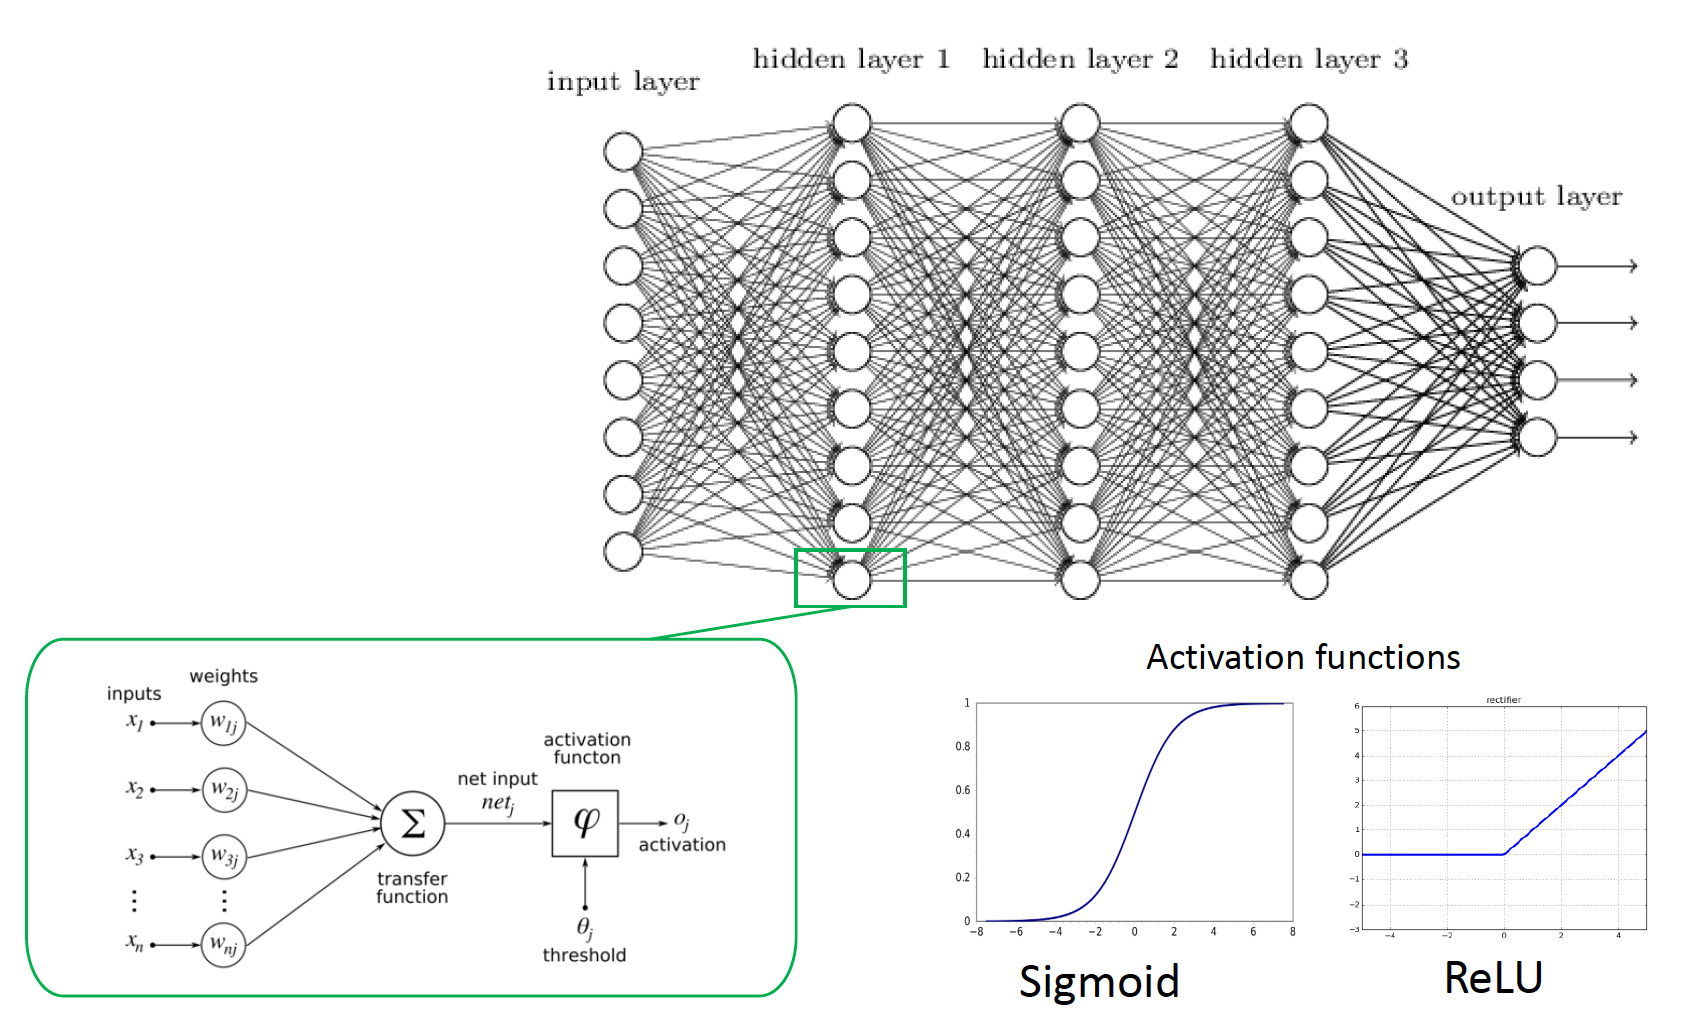
\includegraphics[width=12cm,height=6cm] {ANN.png}}        
    \caption{ANN}      
\end{figure}

This is called fully connected feedforward neural network. Now we want to give a more compressive expression, we collect all the output in $k$-th level $f_{k,l}$ $l = 1,\cdots, L_k$ with $f_{k,L_k+1} = 1$ as a extended vector $\bm{f}_k$. 
So we can have the output in $k+1$-th level under this setting with 
\begin{equation}
    \bm{f}_{k+1}(W_{k+1}) = 
    \begin{pmatrix}
        \bm{g}_{k+1}(\omega_{k+1} \cdot \bm{f}_k(W_k)) \\
        1,
    \end{pmatrix}
\end{equation}
with 
\begin{equation}
    W_{k+1} = \{ \omega_{k+1}, W_k\} \quad \omega_{k+1} \in \mathbb{R}^{(L_{k+1}) \times (L_{k} + 1)},
\end{equation}
and
\begin{equation}
    \bm{g}_{k+1}(x_1,\cdots,x_{L_{k+1}}) = 
    \begin{pmatrix}
        g_{k+1}(x_1) \\ 
        \cdots  \\
        g_{k+1}(x_{L{k+1}})
    \end{pmatrix}
\end{equation}
So at last, we get the final iterative definition with the last output and initial input of this network like:
\begin{equation}
    \begin{cases}
        &\bm{f}_K(W_{K}) = 
        \begin{pmatrix}
            \bm{g}_{K}(\omega_{K} \cdot \bm{f}_{K-1}(W_{K-1})) \\
            1,
        \end{pmatrix} \\
        &\bm{f}_0 = 
        \begin{pmatrix}
            \bm{x} \\
            1
        \end{pmatrix}.
    \end{cases}
\end{equation}
All in all, we can define the tensor similar space like:
\begin{equation}
    T_{3}(\mathcal{L}_K) := \{ \omega_{k,li} \in \mathbb{R}~|~ 1 \le k \le K, 1\le l \le L_k, 1 \le i \le L_{k-1} + 1\}, 
\end{equation}
with 
\begin{equation}
    \mathcal{N}_{K} = (m, L_1, L_2, \cdots, L_{K-1}, c).
\end{equation}
Here we need to mention that, for this kind of deep feedforward neural network, once $\mathcal{N}_K$ is defined we know the whole structure of this network. So we may call $\mathcal{N}_K$ as the network structure parameters. By the way, we have $c = Dim(Y^i) = n_K$ and $m = Dim(X^i) = n_0 $ which are defined by the data and problem properties.

\subsection{Interpolation by optimization}
So the  interpolation process can be seen as a optimization problem in the special function class if the activation function for every elements and  the network structure parameter $\mathcal{N}_K$ are given:
\begin{equation}
    \mathcal{F} = \{\bm{f}_K(W_K;\bm{x}) ~|~  \bm{f}_0 = (\bm{x}^{T},1)^{T}\},
\end{equation}
and the optimization problem can be seen as
\begin{equation}
    %\mathop{\min}_{f \in \mathcal{F}}  \frac{1}{N}\sum_{i=1}^N \|f(X^i) - Y^i\|^2 = 
    \mathop{\min}_{W_K \in T_3(\mathcal{N}_K)}  L(W_K) := \frac{1}{N}\sum_{i=1}^N \|\bm{f}_K(W_K; X^i) - Y^i\|^2.
\end{equation}
But $\mathcal{F}$ this is neither a linear space nor a convex set.




\subsection{Back-Propagation}
Here we will talk about how to compute $\nabla_{W_K} L(W_K)$ by using chain rule which is called BP algorithm in deep learning. By the definition we have:
\begin{equation}
    \nabla_{W_K} L(W_K) = \frac{2}{N} \sum_{i=1}^{N} \nabla_{W_K}\bm{f}_K(W_K; X^i) \cdot (\bm{f}_K(W_K;X^i) - Y^i) . 
\end{equation}
So, the only thing we need to do is to compute $\nabla_{W_K}\bm{f}_K(W_K; X^i)$, if we state this element by element, that is: 
\begin{equation}
    \frac{\partial (\bm{f}_K)_j}{ \partial \omega_{k,l,i}} = \frac{\partial (\bm{f}_K)_j}{\partial \bm{f}_{K-1}} \cdot \frac{ \partial \bm{f}_{K-1}}{\partial \bm{f}_{K-2}} \cdots \frac{ \partial \bm{f}_k}{\partial \omega_{k,l,i}}.
\end{equation}
We can see from the above that, we only need to compute those terms like:
\begin{equation}
    \frac{ \partial \bm{f}_k}{\partial \omega_{k}}  \quad \text{and} \quad \frac{\partial \bm{f}_k}{\partial \bm{f}_{k-1}}  \quad k = 1,2,\cdots,K. 
\end{equation}

Now we are going to derive the expression for every terms, first of all we have $(\bm{f}_k)_{L_k + 1} = 1$, so we have 
$$
\frac{\partial(\bm f_k)_{L_{k} + 1}}{\partial \bm f_{k-1}} = (0,0,\cdots,0) \in \mathbb{R}^{L_{k-1} + 1},
$$
and
$$
\frac{\partial(\bm f_k)}{\partial (\bm f_{k-1})_{L_{k-1}+1}} = (0,0,\cdots,0)^{t} \in \mathbb{R}^{L_{k} + 1}.
$$
To compute $\frac{\partial(\bm f_k)_j}{\partial (\bm f_{k-1})_{l}}$ with $ 1 \le j \le L_k$ and $1 \le l \le L_{k-1}$ we have 
$$
\frac{\partial(\bm f_k)_j}{\partial (\bm f_{k-1})_{l}} = \frac{ g_k( (\omega_k \cdot \bm{f}_{k-1})_j)}{\partial (\bm f_{k-1})_{l}} = g_k'((\omega_k \cdot \bm{f}_{k-1})_j)\omega_{k,jl} .
$$
Combine those results we have:
\begin{equation}\label{eq:partial-f}
    \frac{\partial \bm{f}_k}{\partial \bm{f}_{k-1}} = 
    \begin{pmatrix}
        \omega_{k, (1:n_{k} )\times(1:n_{k-1})} & 0 \\
        0 & 0
    \end{pmatrix}
\end{equation}
The similar results can be derived for $\frac{ \partial \bm{f}_k}{\partial \omega_{k}}$ and we get:
\begin{equation}\label{eq:partial-omega}
    \frac{ \partial (\bm{f}_k)_l}{\partial \omega_{k,ij}} = \begin{cases}
        0 &\text{if} \quad l = L_k + 1\\
        g_k'( \sum_{l,s} \omega_{k,l,s}(\bm{f}_{k-1})_s)\delta_{li}\delta_{js}(\bm{f}_{k-1})_{s} \quad &\text{others}.
    \end{cases}
\end{equation} 

In short, BP algorithm can be expressed as:
\begin{algorithm}[H]
    \begin{algorithmic}[1]
        \STATE {\bf{Input:}}  $X^i$ and $W_K$;
        \FOR{$k = K:-1:1$}
        \STATE Compute and save 
        $$\frac{ \partial \bm{f}_k}{\partial \omega_{k}}  \quad \text{and} \quad \frac{\partial \bm{f}_k}{\partial \bm{f}_{k-1}}$$ by \ref{eq:partial-f} and \ref{eq:partial-omega}
        \STATE Compute 
        $$\frac{ \partial \bm{f}_K}{\partial \omega_{k}} = \frac{\partial \bm{f}_K}{\partial \bm{f}_{K-1}} \cdot \frac{ \partial \bm{f}_{K-1}}{\partial \bm{f}_{K-2}} \cdots \frac{ \partial \bm{f}_k}{\partial \omega_{k}}$$
        \ENDFOR
    \end{algorithmic}
    \caption{Back-Propagation Algorithm}
\end{algorithm}



